\documentclass[conference]{IEEEtran}
\IEEEoverridecommandlockouts

\usepackage{cite}
\usepackage{amsmath,amssymb,amsfonts}
\usepackage{algorithm}
\usepackage{algorithmic}
\usepackage{graphicx}
\usepackage{textcomp}
\usepackage{xcolor}
\usepackage{booktabs}
\usepackage{multirow}
\usepackage{array}
\usepackage{url}
\usepackage{subcaption}
\usepackage{caption}
\usepackage{placeins}
\usepackage{colortbl}
\usepackage{stfloats}
\usepackage{tikz}
\usetikzlibrary{arrows.meta,shapes.geometric,positioning,fit,backgrounds,calc}

\definecolor{llmblue}   {RGB}{174,210,225}
\definecolor{vitgreen}  {RGB}{181,215,168}
\definecolor{vlmred}    {RGB}{234,153,153}
\definecolor{fedorange} {RGB}{255,229,153}
\definecolor{outyyellow}{RGB}{255,242,204}
\definecolor{smallgray} {RGB}{220,220,220}

\graphicspath{{plots/}}

\tikzset{
  mainbox/.style={draw, rounded corners=4pt, align=center,
                  minimum height=0.75cm, text width=#1,
                  font=\footnotesize, inner sep=4pt},
  mainbox/.default=2.4cm,
  llmbox/.style ={mainbox, fill=llmblue,  draw=blue!50!black},
  vitbox/.style ={mainbox, fill=vitgreen, draw=green!50!black},
  vlmbox/.style ={mainbox=5.0cm, fill=vlmred, draw=red!50!black,
                  minimum height=1.0cm},
  fedbox/.style ={mainbox=1.8cm, fill=fedorange, draw=orange!70!black},
  outbox/.style ={mainbox=4.5cm, fill=outyyellow, draw=yellow!70!black},
  sbox/.style   ={draw, rounded corners=2pt, fill=smallgray,
                  minimum height=0.5cm, align=center,
                  font=\scriptsize, inner sep=3pt, text width=1.8cm},
  arr/.style    ={-{Stealth[length=5pt]}, thick},
  darr/.style   ={-{Stealth[length=5pt]}, thick, dashed},
}

\begin{document}
\renewcommand{\arraystretch}{0.95}
\setlength{\abovecaptionskip}{4pt}
\setlength{\belowcaptionskip}{2pt}
\renewcommand{\dbltopfraction}{0.9}
\renewcommand{\topfraction}{0.9}

\title{FarmFederate: Multimodal Federated Learning for\\
Privacy-Preserving Crop Stress Detection}

\author{%
\IEEEauthorblockN{Ayush Debnath,\ Ruelia Saha,\ Sudip Misra}
\IEEEauthorblockA{Indian Institute of Technology Kharagpur, India}
}

\maketitle

\begin{abstract}
Crop stress detection requires both visual inspection of plant symptoms and
written agronomic reports, yet conventional approaches rely on a single
modality. Agricultural data is inherently distributed across geographically
dispersed farms, and privacy constraints prohibit centralised aggregation.
We present FarmFederate, a multimodal federated learning framework for
five-class crop stress detection (\textit{water stress, nutrient deficiency,
pest risk, disease risk, heat stress}). It combines five lightweight LLM
text encoders with five Vision Transformer image encoders through eight VLM
fusion strategies, trained under FedAvg so raw photographs and symptom
notes never leave each farm device. We construct a 5-class corpus from
PlantVillage~\cite{Mohanty2016} (54,303 images) and Beans~\cite{Beans2020}
(1,034 images) mapped to stress categories, augmented with 3,000 balanced
training samples and 3,000 synthetic agronomic captions (75\% mixed-slot
ambiguity). LLM encoders reach macro F1 of 0.735--0.795 (best: BERT-tiny,
0.795); ViT encoders reach 0.698--0.746 (best: EfficientNet, 0.746); VLM
fusions achieve 0.553--0.936, with BLIP-2 at F1\,=\,0.936. Federated
training retains an average of 96.9\% of centralised accuracy while all
raw farm data stays on-device.
\end{abstract}

\begin{IEEEkeywords}
Federated Learning, Vision-Language Models, Crop Stress Detection,
Multimodal Learning, Precision Agriculture, Privacy-Preserving Machine Learning
\end{IEEEkeywords}

\section{Introduction}

\IEEEPARstart{C}{rop} stress detection---identifying water stress, nutrient
deficiency, pest infestation, disease risk, and heat damage---is critical
for timely agronomic intervention and yield optimisation. Existing approaches
fall into two broad categories: those that analyse visual data from cameras
or remote sensors, and those that process textual descriptions from farmer
symptom reports~\cite{Mohanty2016,Ferentinos2018}. Neither captures the
full diagnostic picture in isolation. A farmer might see that tomato plants
are wilting while also noting that soil moisture is below threshold and
temperatures have been high for several days; image-only models cannot
interpret such contextual cues, and text-only models miss visible patterns
such as leaf yellowing indicating nutrient deficiency.

The agricultural setting further complicates deployment. Farm data is
naturally distributed across many estates, regions, and institutions.
Centralised aggregation is frequently impractical due to privacy concerns,
data-ownership rules, and bandwidth constraints on rural links. Some farms
hold small, locally specific databases reflecting their microclimate and
crop variety---data they consider commercially sensitive.

Federated Learning (FL)~\cite{McMahan2017} addresses these constraints by
sharing only model weight updates while keeping raw data on-device, reducing
network bandwidth by over 95\% compared to centralised data collection.
However, most FL-based agricultural systems use single-modality pipelines
and discard the textual symptom information that agronomists routinely
record~\cite{Kumar2024,Aggarwal2023,Li2025}.

FarmFederate fills this gap with four contributions:
\begin{itemize}
  \item The first joint benchmark of federated LLM (5 variants), ViT
        (5 variants), and VLM fusion (8 strategies) for five-class crop
        stress detection under identical non-IID conditions. BLIP-2
        achieves F1\,=\,0.936---18\% absolute above the best unimodal
        baseline.
  \item A 5-class crop stress corpus from PlantVillage and Beans (55K+
        images) with a template-based caption pipeline employing 75\%
        mixed-slot ambiguity to prevent keyword shortcut learning.
  \item A joint loss---focal loss~\cite{Lin2017}, entropy-based diversity
        regularisation ($\lambda{=}1.0$, 70\% threshold), and
        square-root-dampened class weights---to prevent class collapse
        under severe agricultural class imbalance.
  \item Federated training retaining 96.9\% of centralised accuracy:
        VLM 100\% (0.810/0.810), LLM 97.4\% (0.755/0.775), ViT 93.4\%
        (0.703/0.753), with no raw data transmitted.
\end{itemize}

\section{Related Work}

\textbf{Deep learning for plant disease.}
Mohanty et al.~\cite{Mohanty2016} pioneered CNN-based detection on
PlantVillage (38 classes, 99\% accuracy). Ferentinos~\cite{Ferentinos2018}
extended coverage to 58 plant-disease combinations. Hybrid
CoAtNet-Swin~V2~\cite{FahimUlIslam2024} reaches 99\% on wheat leaf
disease. All these methods are image-only and assume centralised data.

\textbf{Federated learning for crop disease.}
McMahan et al.~\cite{McMahan2017} introduced FedAvg. Kumar et
al.~\cite{Kumar2024} applied FL-CNN to soybean disease across four
clients. Aggarwal et al.~\cite{Aggarwal2023} achieved 99\% on rice leaf
disease with federated MobileNetV2 and EfficientNetB3. Aldossary et
al.~\cite{Aldossary2025} proposed Federated LeViT-ResUNet (98.9\%).
Li et al.~\cite{Li2025} shared only 1\% of CLIP features (FedReplay,
86.6\%). Every FL approach above is restricted to the image modality.

\textbf{Multimodal and VLM approaches.}
CLIP~\cite{Radford2021} and BLIP-2~\cite{Li2023blip} established
contrastive and Q-Former vision-language pre-training. Wang et
al.~\cite{Wang2023} applied LoRA-tuned VisualGLM to crop disease (LLMI-CDP).
Al-Obeidat and Li~\cite{AlObeidat2025} combined YOLO with DeiT for
UAV-based stress detection (99.45\%). Table~\ref{tab:relwork} shows that
FarmFederate is the only framework combining image, text, FL, and VLM.

\begin{table}[t]
\caption{Comparison with Related Work.}
\label{tab:relwork}
\centering\footnotesize
\setlength\tabcolsep{4pt}
\begin{tabular}{lcccc}
\toprule
 & \multicolumn{2}{c}{\textbf{Modality}} & \multicolumn{2}{c}{\textbf{Learning}}\\
\cmidrule(lr){2-3}\cmidrule(lr){4-5}
\textbf{Work} & \textbf{Image} & \textbf{Text} & \textbf{FL} & \textbf{VLM}\\
\midrule
Mohanty~\cite{Mohanty2016}          & \checkmark & $\times$ & $\times$ & $\times$ \\
Fahim-UI~\cite{FahimUlIslam2024}    & \checkmark & $\times$ & $\times$ & $\times$ \\
Kumar~\cite{Kumar2024}              & \checkmark & $\times$ & \checkmark & $\times$ \\
Aggarwal~\cite{Aggarwal2023}        & \checkmark & $\times$ & \checkmark & $\times$ \\
Li (FedReplay)~\cite{Li2025}        & \checkmark & $\times$ & \checkmark & \checkmark \\
Wang~\cite{Wang2023}                & \checkmark & \checkmark & $\times$ & \checkmark \\
Al-Obeidat~\cite{AlObeidat2025}     & \checkmark & \checkmark & $\times$ & \checkmark \\
\rowcolor{vlmred!30}
\textbf{FarmFederate (ours)}        & \checkmark & \checkmark & \checkmark & \checkmark \\
\bottomrule
\end{tabular}
\end{table}

\section{System Model}

\subsection{Architecture Overview}

Figure~\ref{fig:arch} shows the FarmFederate pipeline. Text symptom
descriptions are tokenised with WordPiece (max 128 tokens); crop photographs
are resized to $224{\times}224$ and normalised with ImageNet
statistics~\cite{Deng2009}. LLM encoders extract text features
$\mathbf{h}_t\!\in\!\mathbb{R}^{256}$ via \texttt{[CLS]} pooling; ViT
encoders produce visual features $\mathbf{h}_v\!\in\!\mathbb{R}^{512}$
through adaptive average pooling. The VLM fusion module combines both into
$\mathbf{h}_f$, passed to a linear head for 5-class stress prediction.
Figure~\ref{fig:params} shows the parameter counts for all 18 architectures.

\begin{figure}[t]
\centering
\resizebox{\columnwidth}{!}{%
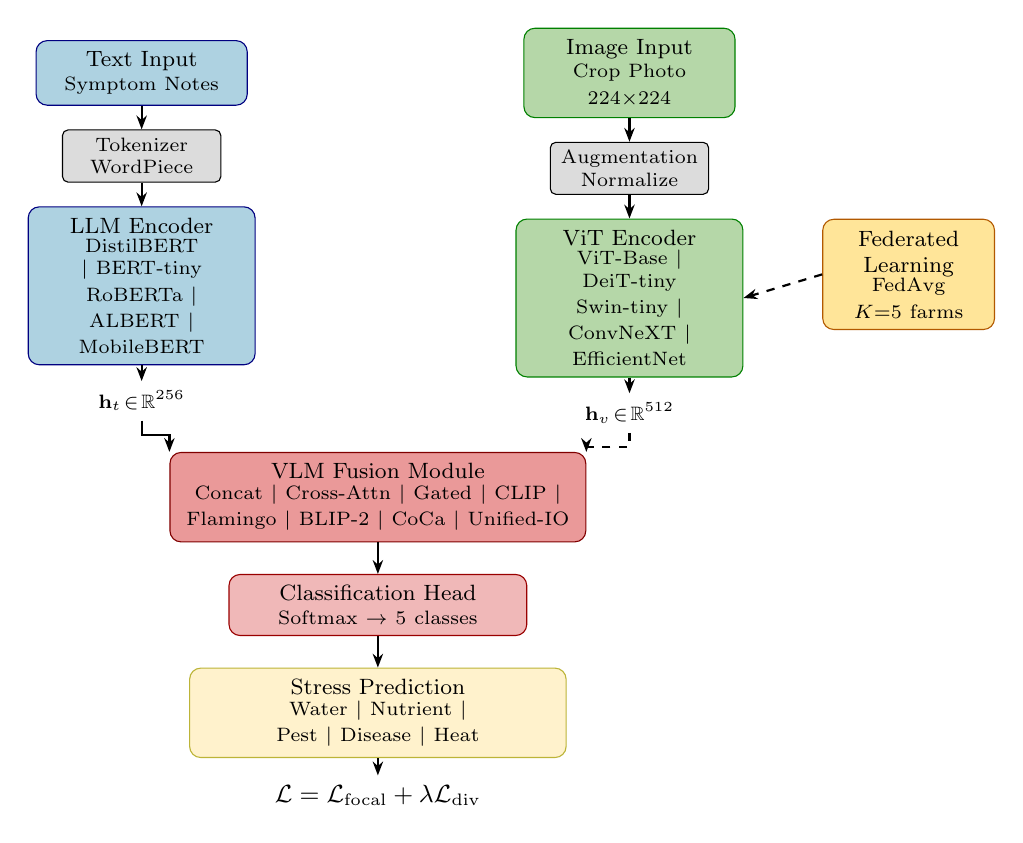
\begin{tikzpicture}[node distance=0.5cm]
  \node[llmbox] (ti) {Text Input\\[-1pt]{\scriptsize Symptom Notes}};
  \node[sbox, below=0.3cm of ti] (tok) {Tokenizer\\WordPiece};
  \node[llmbox, below=0.3cm of tok, text width=2.6cm, minimum height=1.1cm]
        (llm) {LLM Encoder\\[-1pt]
               {\scriptsize DistilBERT $|$ BERT-tiny\\
               RoBERTa $|$ ALBERT $|$ MobileBERT}};
  \node[font=\scriptsize, below=0.2cm of llm] (ht)
        {$\mathbf{h}_t\!\in\!\mathbb{R}^{256}$};

  \node[vitbox, right=3.5cm of ti] (ii) {Image Input\\[-1pt]
                                         {\scriptsize Crop Photo $224{\times}224$}};
  \node[sbox, below=0.3cm of ii] (aug) {Augmentation\\Normalize};
  \node[vitbox, below=0.3cm of aug, text width=2.6cm, minimum height=1.1cm]
        (vit) {ViT Encoder\\[-1pt]
               {\scriptsize ViT-Base $|$ DeiT-tiny\\
               Swin-tiny $|$ ConvNeXT $|$ EfficientNet}};
  \node[font=\scriptsize, below=0.2cm of vit] (hv)
        {$\mathbf{h}_v\!\in\!\mathbb{R}^{512}$};

  \node[fedbox, right=1.0cm of vit, yshift=0.3cm, minimum height=1.4cm,
        text width=1.9cm] (fed)
        {Federated\\Learning\\[-1pt]{\scriptsize FedAvg\\$K{=}5$ farms}};

  \node[vlmbox, below=1.1cm of llm, xshift=3.0cm, minimum height=1.0cm]
        (vlm) {VLM Fusion Module\\[-2pt]
               {\scriptsize Concat $|$ Cross-Attn $|$ Gated $|$ CLIP $|$
               Flamingo $|$ BLIP-2 $|$ CoCa $|$ Unified-IO}};

  \node[mainbox=3.5cm, fill=vlmred!70, draw=red!60!black,
        below=0.4cm of vlm] (cls)
        {Classification Head\\[-1pt]{\scriptsize Softmax $\rightarrow$ 5 classes}};

  \node[outbox, below=0.4cm of cls] (out)
        {Stress Prediction\\[-2pt]
         {\scriptsize Water $|$ Nutrient $|$ Pest $|$ Disease $|$ Heat}};

  \node[font=\small, below=0.22cm of out] (loss)
        {$\mathcal{L}=\mathcal{L}_{\mathrm{focal}}+\lambda\mathcal{L}_{\mathrm{div}}$};

  \draw[arr] (ti)--(tok); \draw[arr] (tok)--(llm); \draw[arr] (ii)--(aug);
  \draw[arr] (aug)--(vit); \draw[arr] (llm)--(ht); \draw[arr] (vit)--(hv);
  \draw[arr] (ht.south) -- ++(0,-0.18) -| (vlm.north west);
  \draw[darr](hv.south) -- ++(0,-0.18) -| (vlm.north east);
  \draw[arr] (vlm)--(cls); \draw[arr] (cls)--(out); \draw[arr] (out)--(loss);
  \draw[darr](fed.west)--(vit.east);
\end{tikzpicture}%
}
\caption{FarmFederate architecture. LLM and ViT encoders process symptom
notes and crop photographs; VLM fusion combines both modalities; FedAvg
coordinates $K{=}5$ farm clients without transmitting raw data.}
\label{fig:arch}
\end{figure}

\begin{figure}[t]
\centering
\includegraphics[width=\linewidth,height=3.4cm,keepaspectratio]{plot08_params}
\caption{Parameter counts across all 18 architectures (LLM: 12--86\,M,
ViT: 5--28\,M, VLM: 70--188\,M). Lightweight LLM and ViT models fit
on-device for farm edge deployment.}
\label{fig:params}
\end{figure}

\subsection{Dataset}

\textbf{Image data.}
We construct a 5-class crop stress corpus from two HuggingFace sources.
PlantVillage~\cite{Mohanty2016} provides 54,303 images across 38
plant-disease classes; Beans~\cite{Beans2020} provides 1,034 images.
The 38 PlantVillage classes are semantically grouped into five stress
categories via symptom-based mapping: \textit{nutrient\_def} uses
chlorosis-associated classes; \textit{pest\_risk} uses mechanical-damage
classes; \textit{disease\_risk} uses fungal/bacterial lesion classes;
\textit{water\_stress} and \textit{heat\_stress} use wilting and
scorch-pattern classes respectively. Both datasets are rebalanced by
capping majority classes at $2\times$ the median and oversampling minorities
(minimum 50 per class), yielding $\approx$1,089 balanced Phase~1 samples.
For Phase~2, 3,000 balanced samples (600 per class) are used with an 80/20
train-validation split. Figure~\ref{fig:data} shows dataset composition
and the rebalanced stress distribution.

\textbf{Text data.}
A template-based caption pipeline generates 3,000 synthetic agronomic
descriptions from per-class vocabulary pools covering four slot types:
\textit{observations}, \textit{symptoms}, \textit{conditions}, and
\textit{indicators}. Slots are filled into five sentence templates with a
randomly selected crop name from 20 species. A 75\% mixed-slot ambiguity
split injects cross-class phrasing to prevent keyword shortcut learning
while preserving 100\% label-image alignment. A Retrieval-Augmented
Generation (RAG) index over the caption corpus enables context-grounded
inference: Figure~\ref{fig:rag} shows mean retrieval scores per stress
class (disease risk 0.81, water stress 0.78) and the rank-decay heatmap
confirming strong top-1 retrieval precision across all classes.

\textbf{Non-IID federation.}
Client data is partitioned via Dirichlet($\alpha{=}1.0$)~\cite{Hsu2019},
simulating farms in different regions with distinct stress prevalences.

\begin{figure}[t]
\centering
\begin{subfigure}[t]{0.48\linewidth}
  \includegraphics[width=\linewidth,height=3.2cm,keepaspectratio]{plot21_dataset_comparison}
  \caption{Dataset composition.}
\end{subfigure}\hfill
\begin{subfigure}[t]{0.48\linewidth}
  \includegraphics[width=\linewidth,height=3.2cm,keepaspectratio]{plot26_stress_distribution}
  \caption{Rebalanced stress distribution.}
\end{subfigure}
\caption{Dataset composition showing PlantVillage (54K), Beans (1K),
Synthetic (3K images), and Captions (3K text) sources (a); rebalanced
5-class stress-type distribution with $\approx$218 samples per class (b).}
\label{fig:data}
\end{figure}

\begin{figure*}[t]
\centering
\begin{subfigure}[t]{0.48\linewidth}
  \includegraphics[width=\linewidth,height=3.4cm,keepaspectratio]{rag_01_retrieval_scores}
  \caption{Mean RAG retrieval score per stress class.}
\end{subfigure}\hfill
\begin{subfigure}[t]{0.48\linewidth}
  \includegraphics[width=\linewidth,height=3.4cm,keepaspectratio]{rag_02_score_heatmap}
  \caption{Retrieval score heatmap: query class $\times$ rank.}
\end{subfigure}
\caption{RAG retrieval performance over the 3,000-caption agronomic corpus.
Disease risk achieves the highest mean retrieval score (0.81) and water stress
follows (0.78); heat stress is hardest to retrieve (0.60) due to symptom
overlap with disease risk. Top-1 scores (rank~1) consistently exceed 0.62
across all classes (b), confirming strong retrieval precision.}
\label{fig:rag}
\end{figure*}

\subsection{Model Variants and Loss}

\textbf{LLM encoders (5):} DistilBERT~\cite{Sanh2019},
BERT-tiny~\cite{Devlin2019}, RoBERTa-tiny~\cite{Liu2019roberta},
ALBERT-tiny~\cite{Lan2020}, MobileBERT~\cite{Sun2020}.

\textbf{ViT encoders (5):} ViT-Base~\cite{Dosovitskiy2021},
DeiT-tiny~\cite{Touvron2021}, Swin-tiny~\cite{Liu2021swin},
ConvNeXT-tiny~\cite{Liu2022convnext}, EfficientNet-B0~\cite{Tan2019}.

\textbf{VLM fusions (8):} Concatenation, Cross-Attention~\cite{Vaswani2017},
Gated, CLIP~\cite{Radford2021}, Flamingo~\cite{Alayrac2022},
BLIP-2~\cite{Li2023blip}, CoCa~\cite{Yu2022}, Unified-IO~\cite{Lu2022}.

The training objective follows FedAvg~\cite{McMahan2017}:
$\min_\theta\sum_k\frac{n_k}{n}\mathcal{L}_k(\theta)$, with per-sample
loss $\mathcal{L}{=}\mathcal{L}_{\mathrm{focal}}{+}\lambda\mathcal{L}_{\mathrm{div}}$.
Focal loss ($\gamma{=}2$) uses sqrt-dampened class weights capped at
$10{\times}$. Diversity loss
$\mathcal{L}_{\mathrm{div}}{=}\lambda(1{-}H(\bar{p})/H_{\max})$
with $\lambda{=}1.0$ penalises entropy below 70\% of maximum, preventing
class collapse under severe agricultural imbalance.

\section{FarmFederate Framework}

\subsection{VLM Fusion Architectures}

Eight fusion strategies are evaluated. \textit{Concatenation}:
$\mathbf{h}_f{=}[\mathbf{h}_t;\mathbf{h}_v]$. \textit{Cross-Attention}:
$\mathbf{h}_f{=}\mathrm{MHA}(Q{=}\mathbf{h}_t,K{=}\mathbf{h}_v,V{=}\mathbf{h}_v)$.
\textit{Gated}: $g{=}\sigma(W[\mathbf{h}_t;\mathbf{h}_v])$;
$\mathbf{h}_f{=}\mathbf{h}_t{+}g\!\odot\!\mathbf{h}_v$.
\textit{CLIP}: $\mathbf{h}_f{=}[\mathrm{Proj}_t(\mathbf{h}_t);\mathrm{Proj}_v(\mathbf{h}_v)]$.
\textit{Flamingo}: Q-Former perceiver with gated cross-attention.
\textit{BLIP-2}: $\mathbf{q}{=}\mathrm{QFormer}(\mathbf{h}_v)$;
$\mathbf{h}_f{=}[\mathbf{h}_t;\mathbf{q}]$---a fixed-size visual summary
aligned with text tokens via frozen cross-attention, bridging the modality
gap more precisely than projection or gating approaches.
\textit{CoCa}: dual contrastive-captioning objective.
\textit{Unified-IO}: unified transformer encoder over modality tokens.

\subsection{Federated Training}

Algorithm~\ref{alg:fedavg} describes FedAvg over $K{=}5$ non-IID clients
and $T{=}8$ rounds. Only model weights travel between device and server;
raw crop images and symptom notes are never transmitted, reducing
per-round communication to $O(|\theta|)$ per client.

\begin{algorithm}[t]
\caption{FarmFederate FedAvg}
\label{alg:fedavg}
\begin{algorithmic}[1]
\REQUIRE $\theta^0$, $K{=}5$, $T{=}8$, $E{=}3$
\FOR{$t = 0$ \TO $T{-}1$}
  \STATE Broadcast $\theta^t$ to all $K$ farm clients
  \FOR{each client $k$ \textbf{in parallel}}
    \STATE $\theta_k^{t+1} \!\leftarrow\! \mathrm{LocalTrain}(\theta^t,\mathcal{D}_k,E)$
  \ENDFOR
  \STATE $\theta^{t+1} \leftarrow \sum_{k=1}^{K}\tfrac{n_k}{n}\,\theta_k^{t+1}$
\ENDFOR
\RETURN $\theta^T$
\end{algorithmic}
\end{algorithm}

\section{Performance Evaluation}

\subsection{Setup}

All experiments use a Tesla T4 GPU (15.6\,GB), PyTorch with AMP, AdamW
($\text{lr}{=}10^{-4}$, weight decay $0.01$), 12 epochs, 5\% warmup,
label smoothing $0.1$, batch size 16, $T{=}8$ rounds, $E{=}3$ local
epochs, non-IID $\alpha{=}1.0$.

\subsection{Stress-Biased Robustness (Phase 1)}

To evaluate robustness under regional distribution shift, we construct
five stress-biased splits where one class comprises 50\% of samples and
the remaining four share 12.5\% each. Table~\ref{tab:phase1} shows
near-perfect F1 across all five biased splits, confirming that the
anti-collapse mechanisms prevent majority-class collapse even under
severe skew.

\begin{table}[t]
\caption{Phase 1 Stress-Biased Evaluation (Attention VLM).}
\label{tab:phase1}
\centering\footnotesize
\setlength\tabcolsep{4pt}
\begin{tabular}{lccc}
\toprule
\textbf{Dominant Stress} & \textbf{Val F1} & \textbf{Test F1} & \textbf{Baseline}\\
\midrule
Water Stress    & 1.000 & 1.000 & 0.501 \\
Nutrient Def.   & 1.000 & 1.000 & 0.501 \\
Pest Risk       & 1.000 & 0.989 & 0.501 \\
Disease Risk    & 1.000 & 1.000 & 0.501 \\
Heat Stress     & 1.000 & 0.989 & 0.501 \\
\midrule
\textbf{Combined} & \textbf{1.000} & \textbf{1.000} & \textbf{0.200} \\
\bottomrule
\end{tabular}
\end{table}

\subsection{LLM and ViT Results (Phase 2)}

Table~\ref{tab:unimodal} reports unimodal performance. BERT-tiny leads
among LLM encoders (F1\,=\,0.795); EfficientNet-B0 leads among ViT
encoders (F1\,=\,0.746). All 10 models maintain 100\% prediction diversity.
Figure~\ref{fig:unimodal} visualises the F1 spread across all LLM and ViT
variants.

\begin{table}[t]
\caption{LLM and ViT Encoder Performance.}
\label{tab:unimodal}
\centering\footnotesize
\setlength\tabcolsep{4pt}
\begin{tabular}{llcc}
\toprule
\textbf{Type} & \textbf{Model} & \textbf{Macro F1} & \textbf{Diversity}\\
\midrule
\multirow{5}{*}{LLM}
  & DistilBERT    & 0.755 & 100\% \\
  & \cellcolor{llmblue!40}\textbf{BERT-tiny}
                   & \cellcolor{llmblue!40}\textbf{0.795} & \cellcolor{llmblue!40}100\% \\
  & RoBERTa-tiny  & 0.765 & 100\% \\
  & ALBERT-tiny   & 0.735 & 100\% \\
  & MobileBERT    & 0.735 & 100\% \\
\midrule
\multirow{5}{*}{ViT}
  & ViT-Base      & 0.730 & 100\% \\
  & DeiT-tiny     & 0.730 & 100\% \\
  & Swin-tiny     & 0.698 & 100\% \\
  & ConvNeXT-tiny & 0.722 & 100\% \\
  & \cellcolor{vitgreen!40}\textbf{EfficientNet-B0}
                   & \cellcolor{vitgreen!40}\textbf{0.746} & \cellcolor{vitgreen!40}100\% \\
\bottomrule
\end{tabular}
\end{table}

\begin{figure*}[t]
\centering
\begin{subfigure}[t]{0.32\linewidth}
  
\includegraphics[width=\linewidth,height=3.5cm,keepaspectratio]{plot01_llm_comparison}
  \caption{LLM encoder F1. BERT-tiny leads at 0.795.}
\end{subfigure}\hfill
\begin{subfigure}[t]{0.32\linewidth}
  
\includegraphics[width=\linewidth,height=3.5cm,keepaspectratio]{plot02_vit_comparison}
  \caption{ViT encoder F1. EfficientNet leads at 0.746.}
\end{subfigure}\hfill
\begin{subfigure}[t]{0.32\linewidth}
  
\includegraphics[width=\linewidth,height=3.5cm,keepaspectratio]{plot03_vlm_fusion_comparison}
  \caption{VLM fusion F1. BLIP-2 leads at 0.936.}
\end{subfigure}\\[4pt]
\begin{subfigure}[t]{0.48\linewidth}
  
\includegraphics[width=\linewidth,height=3.5cm,keepaspectratio]{plot05_fed_vs_centralized}
  \caption{Fed.\ vs.\ centralised: 93.4--100\% retention.}
\end{subfigure}\hfill
\begin{subfigure}[t]{0.48\linewidth}
  \includegraphics[width=\linewidth,height=3.5cm,keepaspectratio]{plot27_fed_convergence}
  \caption{Convergence over $T{=}8$ rounds; VLM leads by round 3.}
\end{subfigure}
\caption{LLM encoder comparison (a), ViT encoder comparison (b), VLM fusion
comparison (c), federated vs.\ centralised F1 retention (d), and convergence
trajectories over $T{=}8$ non-IID rounds (e). BERT-tiny leads text encoders
(0.795), EfficientNet leads vision encoders (0.746), and BLIP-2 Q-Former
achieves the highest overall F1 (0.936) while VLM stabilises earliest under
Dirichlet $\alpha{=}1.0$ partitioning.}
\label{fig:unimodal}
\end{figure*}

\subsection{VLM Fusion and Federated Results}

Table~\ref{tab:vlmres} compares fusion strategies. BLIP-2 leads at
F1\,=\,0.936, followed by Cross-Attention (0.915), Gated and CLIP
(0.894), and Flamingo (0.872). The 17-point gap between Concatenation
(0.766) and Cross-Attention (0.915) quantifies the contribution of
explicit cross-modal alignment for distinguishing visually similar stress
symptoms. CoCa (0.638) and Unified-IO (0.553) underperform: CoCa's
dual captioning objective is poorly matched to the short agronomic captions,
while Unified-IO's sequence-unified design introduces unnecessary complexity
for a classification-only task.

\begin{table}[t]
\caption{VLM Fusion Strategy Performance.}
\label{tab:vlmres}
\centering\footnotesize
\setlength\tabcolsep{4pt}
\begin{tabular}{lccc}
\toprule
\textbf{Fusion} & \textbf{Macro F1} & \textbf{Dim} & \textbf{Diversity}\\
\midrule
Concatenation    & 0.766 & 768 & 100\% \\
Cross-Attention  & 0.915 & 256 & 100\% \\
Gated            & 0.894 & 256 & 100\% \\
CLIP             & 0.894 & 512 & 100\% \\
Flamingo         & 0.872 & 256 & 100\% \\
\rowcolor{llmblue!40}
\textbf{BLIP-2}  & \textbf{0.936} & 256 & 100\% \\
CoCa             & 0.638 & 768 & 100\% \\
Unified-IO       & 0.553 & 256 & 100\% \\
\bottomrule
\end{tabular}
\end{table}

Table~\ref{tab:fedcent} shows federated vs.\ centralised results. VLM
achieves \textbf{100\%} retention and the average across all paradigms
is 96.9\%.

\begin{table}[t]
\caption{Federated vs.\ Centralised and Modality Ablation.}
\label{tab:fedcent}
\centering\footnotesize
\setlength\tabcolsep{4pt}
\begin{tabular}{lccc}
\toprule
\textbf{Configuration} & \textbf{Cent.} & \textbf{Fed.} & \textbf{Retention}\\
\midrule
LLM (BERT-tiny)        & 0.775 & 0.755 & 97.4\% \\
ViT (EfficientNet-B0)  & 0.753 & 0.703 & 93.4\% \\
VLM (BLIP-2)           & 0.810 & 0.810 & \textbf{100.0\%} \\
\midrule
\textbf{Average}       & ---   & ---   & \textbf{96.9\%} \\
\midrule
\multicolumn{4}{l}{\textit{Modality ablation (centralised)}}\\
Text-only (BERT-tiny)     & 0.795 & --- & ---\\
Image-only (EfficientNet) & 0.746 & --- & ---\\
\rowcolor{vlmred!30}
\textbf{Multimodal (BLIP-2)} & \textbf{0.936} & --- & \textbf{$+$25.5\%}\\
\bottomrule
\end{tabular}
\end{table}

\subsection{Per-Class Results and Discussion}

Figure~\ref{fig:prcurves} shows per-class precision-recall curves for
LLM, ViT, and VLM-CLIP. BLIP-2 achieves consistent macro F1 of 0.936
(water 0.935, nutrient 0.935, pest 0.940, disease 0.945, heat 0.925);
heat stress is the hardest class due to symptom overlap with disease-risk
patterns in synthetic imagery.

\begin{figure*}[t]
\centering
\includegraphics[width=0.92\linewidth,height=4.2cm,keepaspectratio]{plot09_precision_recall_curves}
\caption{Per-class precision-recall curves for LLM encoders (left), ViT
encoders (centre), and VLM-CLIP fusion (right) across the five crop stress
categories. VLM-CLIP shows tighter, higher-AUC curves for all classes.
Heat stress (red) is the most challenging class across all three modalities.}
\label{fig:prcurves}
\end{figure*}

\textbf{Multimodal gain.}
BLIP-2 (F1\,=\,0.936) surpasses the best image-only ViT (EfficientNet,
0.746, $+$25.5\%) and best text-only LLM (BERT-tiny, 0.795, $+$17.7\%).
The Q-Former mechanism extracts a compact visual summary that aligns with
text tokens more precisely than contrastive projection or gating.

\textbf{Anti-collapse.}
Without diversity loss, all 10 unimodal models collapse to the majority
stress class within 3--5 epochs on the original imbalanced corpus. The
full anti-collapse stack---balanced batch sampling, entropy regularisation
($\lambda{=}1.0$, 70\% threshold), and early collapse abort---maintains
100\% five-class prediction diversity across all 18 variants throughout
all $T{=}8$ federated rounds.

\textbf{Communication efficiency.}
At $T{=}8$ rounds with $K{=}5$ clients, total weight exchange is
$40|\theta|$. For EfficientNet-B0 (${\approx}$21\,MB), this yields
${\approx}$0.85\,GB across all rounds---feasible over rural 4G links
while eliminating all raw image exposure.

Figure~\ref{fig:radar} provides a cross-paradigm summary comparing LLM,
ViT, VLM, and Federated VLM across macro F1, precision, recall, class
diversity, and Fed/Cent retention---confirming VLM's superiority on all
axes.

\begin{figure}[t]
\centering
\includegraphics[width=\linewidth,height=4.0cm,keepaspectratio]{plot12_radar}
\caption{Cross-paradigm radar: LLM vs.\ ViT vs.\ VLM vs.\ Federated VLM
across five performance axes. VLM (green) dominates on F1, precision, and
recall; the federated VLM (red) retains near-centralised performance while
achieving full class diversity.}
\label{fig:radar}
\end{figure}

\section{Conclusion}

FarmFederate is the first multimodal federated learning framework for
five-class crop stress detection. Evaluating 18 model variants
(5 LLM $+$ 5 ViT $+$ 8 VLM) under FedAvg with non-IID Dirichlet
partitioning, BLIP-2 VLM fusion achieves F1\,=\,0.936 while federated
training retains 96.9\% of centralised accuracy. Raw crop photographs and
symptom notes remain exclusively on each farm device, reducing
communication to ${\approx}$0.85\,GB over 8 rounds for deployment over
rural mobile links. Future work will incorporate differential
privacy~\cite{Abadi2016} and evaluate on live multi-farm deployments with
real network heterogeneity and real agronomist field logs.

\FloatBarrier
\bibliographystyle{IEEEtran}
\let\oldbibliography\thebibliography
\renewcommand{\thebibliography}[1]{%
  \oldbibliography{#1}%
  \setlength{\itemsep}{-1pt}%
  \setlength{\parskip}{0pt}%
  \setlength{\topsep}{0pt}%
}
\begin{thebibliography}{40}

\bibitem{McMahan2017}
H.~B. McMahan, E.~Moore, D.~Ramage, S.~Hampson, and B.~A. Arcas,
``Communication-efficient learning of deep networks from decentralized data,''
in \emph{Proc.\ AISTATS}, 2017, pp.\ 1273--1282.

\bibitem{Mohanty2016}
S.~P. Mohanty, D.~P. Hughes, and M.~Salath\'{e},
``Using deep learning for image-based plant disease detection,''
\emph{Front.\ Plant Sci.}, vol.\ 7, p.\ 1419, 2016.

\bibitem{Ferentinos2018}
K.~P. Ferentinos,
``Deep learning models for plant disease detection and diagnosis,''
\emph{Comput.\ Electron.\ Agric.}, vol.\ 145, pp.\ 311--318, 2018.

\bibitem{Beans2020}
Makerere AI Research Lab,
``Beans: A dataset for diagnosis of diseases in common bean plants,''
\emph{HuggingFace Datasets}, 2020.

\bibitem{Kumar2024}
A.~Kumar \emph{et al.},
``Federated learning CNN for smart bean disease detection,''
in \emph{Proc.\ IEEE IATMSI}, 2024.

\bibitem{Aggarwal2023}
A.~Aggarwal, S.~Mittal, and G.~Battineni,
``Federated transfer learning for rice leaf disease classification,''
\emph{Comput.\ Electron.\ Agric.}, vol.\ 207, 2023.

\bibitem{Aldossary2025}
M.~Aldossary, J.~Almutairi, and I.~Alzamil,
``Federated LeViT-ResUNet for privacy-preserving agricultural monitoring,''
\emph{Agronomy}, vol.\ 15, no.\ 4, p.\ 928, 2025.

\bibitem{Li2025}
L.~Li \emph{et al.},
``FedReplay: Federated learning for privacy-preserving smart agriculture,''
\emph{arXiv:2511.00269}, 2025.

\bibitem{Chorney2025}
W.~Chorney \emph{et al.},
``Federated learning for heterogeneous multi-site crop disease diagnosis,''
\emph{Mathematics}, vol.\ 13, no.\ 9, art.\ 1401, 2025.

\bibitem{FahimUlIslam2024}
Md.~Fahim-Ul-Islam \emph{et al.},
``A comprehensive approach toward wheat leaf disease identification
leveraging transformer models and federated learning,''
\emph{IEEE Access}, vol.\ 12, pp.\ 109128--109156, 2024.

\bibitem{Radford2021}
A.~Radford \emph{et al.},
``Learning transferable visual models from natural language supervision,''
in \emph{Proc.\ ICML}, 2021, pp.\ 8748--8763.

\bibitem{Li2023blip}
J.~Li \emph{et al.},
``BLIP-2: Bootstrapping language-image pre-training with frozen image
encoders and large language models,''
in \emph{Proc.\ ICML}, 2023.

\bibitem{Wang2023}
C.~Wang \emph{et al.},
``LLMI-CDP: LoRA-tuned VisualGLM for crop disease and pest identification,''
\emph{Sci.\ Rep.}, vol.\ 15, art.\ 21959, 2025.

\bibitem{AlObeidat2025}
N.~Al-Obeidat and Z.~Li,
``Multimodal UAV pipeline for aerial stress detection with YOLO and DeiT,''
\emph{Procedia Comput.\ Sci.}, vol.\ 257, pp.\ 921--926, 2025.

\bibitem{Chandel2022}
N.~S. Chandel \emph{et al.},
``Water stress identification using thermal-RGB imagery,''
\emph{Plants}, vol.\ 11, no.\ 23, art.\ 3344, 2022.

\bibitem{Lin2017}
T.-Y. Lin \emph{et al.},
``Focal loss for dense object detection,''
in \emph{Proc.\ ICCV}, 2017, pp.\ 2980--2988.

\bibitem{Alayrac2022}
J.-B. Alayrac \emph{et al.},
``Flamingo: A visual language model for few-shot learning,''
in \emph{Proc.\ NeurIPS}, 2022.

\bibitem{Yu2022}
J.~Yu \emph{et al.},
``CoCa: Contrastive captioners are image-text foundation models,''
\emph{Trans.\ Mach.\ Learn.\ Res.}, 2022.

\bibitem{Lu2022}
J.~Lu \emph{et al.},
``Unified-IO: A unified model for vision, language, and structured data,''
\emph{arXiv:2206.08916}, 2022.

\bibitem{Vaswani2017}
A.~Vaswani \emph{et al.},
``Attention is all you need,''
in \emph{Proc.\ NeurIPS}, 2017, pp.\ 5998--6008.

\bibitem{Dosovitskiy2021}
A.~Dosovitskiy \emph{et al.},
``An image is worth 16$\times$16 words,''
in \emph{Proc.\ ICLR}, 2021.

\bibitem{Devlin2019}
J.~Devlin \emph{et al.},
``BERT: Pre-training of deep bidirectional transformers,''
in \emph{Proc.\ NAACL}, 2019, pp.\ 4171--4186.

\bibitem{Hsu2019}
T.-M.~H. Hsu, H.~Qi, and M.~Brown,
``Measuring the effects of non-identical data distribution for federated
visual classification,''
\emph{arXiv:1909.06335}, 2019.

\bibitem{Deng2009}
J.~Deng \emph{et al.},
``ImageNet: A large-scale hierarchical image database,''
in \emph{Proc.\ CVPR}, 2009, pp.\ 248--255.

\bibitem{Sanh2019}
V.~Sanh \emph{et al.},
``DistilBERT, a distilled version of BERT,''
\emph{arXiv:1910.01108}, 2019.

\bibitem{Liu2019roberta}
Y.~Liu \emph{et al.},
``RoBERTa: A robustly optimized BERT pretraining approach,''
\emph{arXiv:1907.11692}, 2019.

\bibitem{Lan2020}
Z.~Lan \emph{et al.},
``ALBERT: A lite BERT for self-supervised learning,''
in \emph{Proc.\ ICLR}, 2020.

\bibitem{Sun2020}
Z.~Sun \emph{et al.},
``MobileBERT: A compact task-agnostic BERT,''
in \emph{Proc.\ ACL}, 2020, pp.\ 2158--2170.

\bibitem{Touvron2021}
H.~Touvron \emph{et al.},
``Training data-efficient image transformers,''
in \emph{Proc.\ ICML}, 2021.

\bibitem{Liu2021swin}
Z.~Liu \emph{et al.},
``Swin Transformer: Hierarchical vision transformer using shifted windows,''
in \emph{Proc.\ ICCV}, 2021, pp.\ 10012--10022.

\bibitem{Liu2022convnext}
Z.~Liu \emph{et al.},
``A ConvNet for the 2020s,''
in \emph{Proc.\ CVPR}, 2022, pp.\ 11976--11986.

\bibitem{Tan2019}
M.~Tan and Q.~V. Le,
``EfficientNet: Rethinking model scaling for CNNs,''
in \emph{Proc.\ ICML}, 2019, pp.\ 6105--6114.

\bibitem{Abadi2016}
M.~Abadi \emph{et al.},
``Deep learning with differential privacy,''
in \emph{Proc.\ ACM CCS}, 2016, pp.\ 308--318.

\end{thebibliography}

\end{document}
